\documentclass[10pt,twocolumn,letterpaper]{article}

\usepackage{booktabs}
% \usepackage{caption}
% \captionsetup[table]{skip=8pt}   % केवल तालिकाहरूमा प्रभाव पार्छ
\usepackage{stfloats}  % यो प्रिएम्बलमा थप्नुहोस्
\usepackage{float}
% \usepackage[T1]{fontenc}

%–– line-breaking for Nepali (uses spaces, but set locale if you want hyphenation patterns) ––
% \XeTeXlinebreaklocale "ne"
% \XeTeXlinebreakskip = 0pt plus 1pt

\usepackage{fontspec}
\usepackage{ucharclasses}

%–– define your two fonts ––
\newfontfamily\latinfont{Latin Modern Roman}              % for all non-Devanagari text
% \newfontfamily\nepalifont[Script=Devanagari]{Noto Serif Devanagari}    % for all Nepali text; change “Phobikha” to your font’s exact name
\newfontfamily\nepalifont[Script=Devanagari]{Noto Sans Devanagari}    % for 

%–– ucharclasses auto-detects Unicode blocks ––
\setDefaultTransitions{\latinfont}{}                      
\setTransitionsForDevanagari{\nepalifont}{\latinfont}   % switch to Nepali font in Devanagari, then back
\setTransitionTo{DevanagariDanDa}{\nepalifont}



\usepackage{cvpr}
\usepackage{times}
\usepackage{epsfig}
\usepackage{graphicx}
\usepackage{amsmath}
\usepackage{amssymb}


\usepackage[breaklinks=true,bookmarks=false]{hyperref}

\cvprfinalcopy % *** अन्तिम पेशका लागि यो लाइन अनकमेण्ट गर्नुहोस्
\def\cvprPaperID{****} % *** यहाँ CVPR Paper ID प्रविष्ट गर्नुहोस्
\def\httilde{\mbox{\tt\raisebox{-.5ex}{\symbol{126}}}}

% \renewcommand{\tablename}{ตาราง}
% \renewcommand{\figurename}{รูปที่}   % or whatever you like instead of "Hình"
% \renewcommand{\refname}{เอกสารอ้างอิง}

% \makeatletter
% \def\abstract{%
%   \centerline{\large\bf บทคัดย่อ}% <-- your new label
%   \vspace*{12pt}%
%   \it%
% }
% \makeatother

% This makes the font slightly bigger than base (10) and bold in Subsection headings rather than using ptmb
\makeatletter
\def\cvprsubsection{%
  \@startsection{subsection}{2}{\z@}%
    {8pt plus 2pt minus 2pt}{6pt}%
    % {\normalfont\bfseries\selectfont}%
    {\normalfont\bfseries\fontsize{11}{13}\selectfont}%
}
\makeatother

% So this hardcodes the style for the numbers in the section/subsection headings so they're bold
\font\elvbf=ptmb scaled 1100
\font\elvbfs=ptmb scaled 1200
\makeatletter
% Section number: Large + bold
\renewcommand\thesection{%
  {\elvbfs\arabic{section}}%
}

% Subsection number: normalsize + bold + custom punctuation
\renewcommand\thesubsection{%
  {\elvbf
   \arabic{section}.\arabic{subsection}}%
}
\makeatother

% पृष्ठहरू सबमिशन मोडमा क्रमांकित छन्, र क्यामेरा-रेडीमा बिना नम्बर
%\ifcvprfinal\pagestyle{empty}\fi
\setcounter{page}{1}
\begin{document}

%%%%%%%%% शीर्षक
\title{ECDO डेटा-ड्रिवेन प्राइमर भाग १/२: एक्सोथर्मिक कोर-म्यान्टल डिसप्लिङ्ग ज्यानिबेकोभक् दोलन (ECDO) “पृथ्वी पल्टिने” सिद्धान्तको वर्तमान बुझाइ}

\author{जुनहो\\
प्रकाशित फेब्रुअरी २०२५\\
वेबसाइट (यहाँबाट कागजातहरू डाउनलोड गर्नुहोस्): \href{https://sovrynn.github.io}{sovrynn.github.io}\\
ECDO अनुसन्धान रिपोजिटरी: \href{https://github.com/sovrynn/ecdo}{github.com/sovrynn/ecdo}\\
{\tt\small junhobtc@proton.me}
}

\maketitle
%\thispagestyle{empty}

\begin{abstract}
मे २०२४ मा, "The Ethical Skeptic” \cite{0} नामक छद्म नाममा एक अनलाइन लेखकले Exothermic Core-Mantle Decoupling Dzhanibekov Oscillation (ECDO) \cite{1} नामक एक क्रान्तिकारी सिद्धान्त साझा गरे। यस सिद्धान्तले पृथ्वीको घुम्ने अक्षमा अप्रत्याशित, विनाशकारी परिवर्तनहरू पहिले भइसकेको भन्ने सुझाव दिन्छ, जसले पृथ्वीको घूर्णन जडत्वका कारण महासागरहरूले महादेशहरूमा फैलंदै ठूला विश्वव्यापी बाढीहरू ल्याएका थिए। साथै, यसमा एउटा स्पष्टीकरणात्मक भूभौतिकीय प्रक्रिया र तथ्याङ्कहरू प्रस्तुत गरिएको छ, जसले यस्तो अर्को उल्टो घटना नजिकै हुनसक्ने सङ्केत गर्छ। यस किसिमका प्रलयकारी बाढी तथा विनाशसम्बन्धी भविष्यवाणीहरू नयाँ होइनन्, तर ECDO सिद्धान्त वैज्ञानिक, आधुनिक, बहुविषयगत तथा तथ्याङ्क-आधारित नजिकिएर अनुपम रूपमा आकर्षक छ।

यो लेख ECDO सिद्धान्तमा आधारित छ महिनाको स्वतन्त्र अनुसन्धान \cite{2,20} को दुई-भागको संक्षिप्त सारांशको पहिलो भाग हो। यसले तीन प्रमुख बुँदाहरूलाई उजागर गर्छः

\begin{flushleft}
\begin{enumerate}
    \item बाढीका मिथकहरू र विशाल महादेशीय बाढीका भूवैज्ञानिक सङ्केतहरूले देखाउँछ कि मानव सभ्यताको हालैको इतिहासमा ECDO-जस्तो 'पृथ्वीको उल्टो' पटकौं पटक भएको छ।

\item विगतका पृथ्वी पल्टिने घटनाहरूको अनुमानित दिशा र परिमाण निर्धारण गर्न सकिन्छ।
\item हालका भूचुम्बकीय र भू-भौतिक तथ्याङ्कहरूले अर्को पृथ्वी पल्टिने घटना नजिकै हुन सक्ने संकेत गर्छन्, र वातावरणीय परिवर्तन मानवका कारण नभई पृथ्वीको गहिराइमा भएका परिर्वतनहरूले हुन सक्ने सम्भावना रहेको सुझाव दिन्छ।
\end{enumerate}
\end{flushleft}

अझै म ECDO सिद्धान्तद्वारा प्रस्तावित “पृथ्वी पल्टिने” को कारण हुने भौतिकशास्त्रको विषयमा चर्चा गर्दछु।

यो लेखमा, म कठोर डाटामा केन्द्रित भई वस्तुनिष्ठ रहने, आकर्षक तर अनुमानित भागहरूलाई जोगाउने, र मानवजातिले यस विषयमा थप अनुसन्धान गर्न अत्यन्त जरुरी रहेकोमा जोड दिने प्रयास गर्दछु।
\end{abstract}
\section{परिचय}

महान बाढीका कथाहरू नयाँ होइनन् - वास्तवमा, ती विश्वका सबै प्रमुख संस्कृतिमा पाइन्छन्, सभ्यताको सबै उद्गमस्थलहरूमा फैलिएका छन्। २६७ वटा बाढीका कथाहरूको एक संकलन (चित्र \ref{fig:1}) प्लट गर्दा \cite{3} देखिन्छ कि प्रायः बसोबास योग्य पृथ्वीका सबै क्षेत्रमा बाढीका कथाहरू भेटिन्छन्।

\begin{figure}[h]
\begin{center}
% \fbox{\rule{0pt}{2in} \rule{0.9\linewidth}{0pt}}
   \includegraphics[width=1\linewidth]{b.png}
\end{center}
   \caption{विश्वभरका बाढीका कथाहरूका स्थानहरू \cite{3}.}
\label{fig:1}
\label{fig:onecol}
\end{figure}

यी बाढीका कथाहरूलाई नजिकबाट हेर्दा देखिन्छ कि यी सामान्य बाढीहरू थिएनन्, बरु, ध्वंसात्मक प्रलयहरू थिए जसमा बाढीहरू आएका थिए जसले महादेशहरूलाई सफा बनाए।

\subsection{स्वदेशी अमेरिकी प्रलयका कथाहरू}

स्वदेशी अमेरिकी कथाहरूमा पृथ्वीका ठूला प्रलयहरूको सबैभन्दा जीवित वर्णन समावेश छन्। होपी, एक स्वदेशी अमेरिकी जाति जसले उत्तरपूर्वी अरिजोनामा बसोबास गर्छ, भन्छन्, \textit{"..सोटुक्नाङले छानीएका मानिसहरूको लागि कमिला मानिसहरूलाई आफ्नो भूमिगत संसार खोल्न बोलाए। जब उनीहरू सुरक्षित रूपमा भूमिगत पुगे, सोटुक्नाङले जुम्ल्याहा, पोकाङहोया र पलोङावहोयालाई, जसलाई संसारको ध्रुवको उत्तर र दक्षिणको टुप्पोमा पृथ्वीलाई सही रूपमा घुमाउन राखिएको थियो, आफ्नो स्थान छोड्न आदेश दिए। \textbf{जुम्ल्याहाहरूले आफ्नो स्थान छोड्नासाथ पृथ्वी, नियन्त्रण गर्ने कोही नभएकाले, असन्तुलित भयो, पागलझैँ घुम्यो, अनि दुईपटक पल्टियो।} डाँडाहरू ठूलो छप्कसँग समुद्रमा खसे, समुद्र र तालहरूले जमिनमा बग्यो; जब पृथ्वी चिसो र निर्जीव अन्तरिक्ष भित्र घुम्थ्यो, त्यो कडा बरफमा जम्यो"} \cite{4}.
Many of these stories precisely describe the massive scale of flooding, recounting how the oceans rose to submerge all but the highest mountain peaks. The Skokomish Indians, living in Washington state, tell how, \textit{"महान आत्माले, मानिस र जनावरहरूको दुष्टतासँग रिसाएपछि, धरतीबाट सबै जनावर र मानिस, एउटा असल मानिस र उसको परिवार बाहेक, हटाउने निर्णय गर्यो। महान आत्माको निर्देशनमा, मानिसले बादलमा एउटा बाण प्रहार गर्यो, अनि अर्को बाण त्यो बाणमा, यसरी गर्दै, बादलदेखि जमिनसम्म बाणको डोरी बनायो। असल जनावर र मानिसहरू माथि चढे। नराम्रो जनावर र सर्पहरू चढ्न थाले, तर मानिसले डोरी काटिदियो। \textbf{त्यसपछि महान आत्माले धेरै दिनसम्म वर्षा गरायो, जसले ताखोमा (माउन्ट रेनीयर) को हिउँको लाइनसम्म बाढी ल्यायो।} सबै नराम्रो मानिस र जनावरहरू डुबाएर मरेपछि, महान आत्माले वर्षा रोके, पानी विस्तारै घट्यो, असल मानिस र जनावरहरू तल झरे"} \cite{3}। जानकारीको लागि, माउन्ट रेनीयर वाशिङ्टन राज्यको एउटा सक्रिय ज्वालामुखी हो, जसको शिखर समुद्र सतहदेखि ४३९२.५ मीटर उचाइमा छ।

वाशिङ्टन राज्यका माखा आदिवासीहरूको बाढी कथाले विशेषगरी बाढीको "धेरै न्यानो" पानी भएको बहु-चरणको बाढीको उल्लेख गर्छ, जसको अर्थ यो साधारण बाढी थिएन: \textit{"समुन्द्र यति उच्च उठ्यो कि केपलाई काट्यो। त्यसपछि चार दिनपछि पानी घटेर निया उपत्यका उजाड भयो। फेरि पानी बढ्यो र सबैजसो पहाडका टाकुरा बाहेक डुबायो। \textbf{उठ्दै गएको पानी निकै न्यानो थियो।} डुङ्गामा आफ्ना सामान हालेर मानिसहरू टाढा उत्तरतर्फ चढाइँए। धेरैजना रूखमा डुङ्गा अड्किँदा मरे। फेरि चार दिनपछि समुद्र सामान्य अवस्थामा फर्कियो, अनि मानिसहरू आफूलाई धेरै टाढा उत्तरमा भेटे, जहाँ अहिले पनि तिनीहरूका सन्तानहरू बाँचिरहेका छन्"} \cite{3}।

\subsection{चिनियाँ महाप्रलयका कथाहरू}

प्रशान्त महासागरको अर्को छेउमा, आधुनिक चिनियाँ सभ्यता एउटा ठूलो बाढीसँगै सुरु भएको भनिन्छ। झिया राजवंश, जसको अवस्थित सन् २००० ईसा पूर्वतिर अनुमान छ, यू महानद्वारा स्थापना गरिएको थियो, जसले गुन-यू को महाबाढी रोक्यो \cite{6}। उनको समयमा, \textit{"... चमत्कार भन्न मिल्ने कुरा भयो कि सुर्य दस दिनसम्म अस्ताएन, वनहरूमा आगो बल्यो, र धेरैखाले घिनलाग्दा किराहरू धेरै जन्मिए... एउटा विशाल छाल “आकाशसम्म पुगेको” चीन भूमिमा खस्यो। \textbf{"पानी पहाडका उच्च शिखरसम्म आइपुग्यो, अनि फेदीहरू केही देखिएनन्"}... “डुबानमा बगेका पानीहरू विनाशकारी छन्,” सम्राटले भन्नुभयो। “यिनीहरू यति धेरै फैलिएका छन् कि पहाडहरूलाई घेरेर अग्ला स्थानहरू समेत पुरेर, आफ्नो बाढीसँग स्वर्गलाई नै धम्की दिएका छन्।” सम्राटले आदेश दिए कि डुबेका पानीहरूलाई पहाडका बीचको उपत्यकाबाट निकाल्न सबै प्रयास गरियोस्। धेरै वर्षसम्म जनसंख्याले जस्तोसुकै प्रयास गरेर पनि उपत्यका र मैदानलाई पानीमुक्त पार्न च्यानल खनेर जमिन सुकाउने प्रयास गर्‍यो। धेरै वर्षसम्म सबै प्रयास व्यर्थ भए। यस विशाल कार्यका जिम्मेवार मन्त्री ख्वानलाई असफल भएकाले मृत्युदण्ड दिइयो... र अन्ततः उनका छोरा युले मात्र जमिन सुकाउन सफल भए। उनको उपलब्धि यति महान मानियो कि यु स्युन राजा पश्चात, याहाउका उत्तराधिकारीको रूपमा चीनका सम्राट बने"} \cite{5}।

यसबाट यस्तो देखिन्छ कि चीनमा मात्र बाढी आएको थिएन, तर दिशा चिन्न र सूर्य चन्द्रमाको चाल नाप्न समेत नयाँ हिसाब चाहियो, जसले पृथ्वीको घुम्ने ढाँचा पनि सायद बाढीका बेला बदलिए जस्तो देखाउँछ: \textit{\textbf{"यस सम्राटले विद्वानहरूलाई चीनका विभिन्न भागमा, इन्डो-चीनसम्म पठाएर, सूर्यको उदयअस्त र ताराहरूको चाल हेरेर उत्तर, पश्चिम, पूर्व, दक्षिण फेला पार्न लगाए।} उनले आफ्ना ज्योतिषीहरूलाई ऋतुसमयको अवधि पत्ता लगाउन र नयाँ पात्रो बनाउन पनि आदेश गरे... “त्यसपछि याओ (याहाउ) ले हे र होलाई, विशाल आकाश अनुसार, सुर्य, चन्द्रमा, तारा, र राशिचक्रका चाल र स्वरूप गणना गराउने, राशि परिचय गराउने अनि सम्मानपूर्वक ऋतु जनतालाई सूचित गराउने जिम्मा लगाए”"} \cite{5}।
Records of cataclysms in Chinese history actually date back long before the Xia Dynasty, reaching as early as the Three Sovereigns and Five Emperors period \cite{7}. Nüwa, one of the Three Sovereigns and a central Creation figure in Chinese history, stopped the flood during a cataclysm where the Earth changed rotation: \textit{"दुई शक्तिशाली देवताहरुबीच झगडा भयो, र उनीहरूले युद्ध गरेर टुंग्याउने निर्णय गरे। जल देवता Gong Gong ले आफू हार्दै गरेको देखेपछि, उसले आकाशलाई थाम्ने स्तम्भ पर्वत Buzhou सँग आफ्नो टाउको ठोक्यो। \textbf{स्तम्भ ढल्यो र यसले आकाश उत्तरपश्चिम तिर झुकेको र पृथ्वी दक्षिणपूर्व तिर सरेको कारण बन्यो।} यसले ठूलो विपत्ति ल्यायो, जस्तै कहिल्यै नसकिने आगो, विशाल बाढी, र डर लाग्दा मानिस खाने जनावरहरुको उपस्थिति। Nüwa ले ठूलो कछुवाको खुट्टा काटेर ढलेको स्तम्भको ठाउँमा राखिन्, अवस्था सुधारिन् र सात रङ्गका ढुंगाले फुटेको आकाश सिलाइन्, तर उनी पूर्ण रूपमा झुकेको आकाश ठिक गर्न सकिनन्"} \cite{8}।

\subsection{युरोपेली, माया, मध्य पूर्वी, र दक्षिणपूर्वी एशियाली प्रलयका कथाहरू}

यस कागजातभित्र सबै प्रलयका कथाहरूको विवरण दिन अत्यन्तै धेरै कथाहरू भएकाले, मैले यस्ता कथाहरू भएका उल्लेखनीय अरू केही संस्कृतिहरूको संक्षिप्त उल्लेख मात्रै गर्नेछु। ग्रीक साहित्यमा ड्यूक्यालियन, ओग्यजस, र डार्डानसको प्रलय कथा छन् \cite{9,10}। पहिलोलाई लिएर, \textit{"नौ दिनको बाढीपछि, संसार नष्ट भयो, र डुँगा पर्वत Parnassusको शिखरमा अडियो"}, जसको उच्चतम उचाइ २,४५७ मिटर छ \cite{11}। माया साहित्यका अनुसार अहिलेको सूर्यभन्दा पहिले चारवटा पृथक सूर्य थिए, र चौथो सूर्य Calchiuhtlicue को युग झण्डै ३१०० ई.पू. मा संसार-विनाशक प्रलयसँगै समाप्त भयो र अहिलेको पाँचौं सूर्यको जन्म भयो \cite{12}। मध्यपूर्वमा, बाइबलीय कालक्रममा नोआको प्रख्यात जलप्रलय समावेश छ, र बेबिलोनियन कविता Epic of Gilgamesh ले पनि यस्तै कथा भन्छ \cite{13}। दक्षिणपूर्वी एशियाली संस्कृतिहरूमा पनि प्रलयका कथाहरू धनी छन् - उदाहरणका लागि, इन्डोनेसियाका Ot Danum समुदाय भन्छन्, \textit{"एक ठूलो बाढीले धेरै मानिसहरूलाई डुबायो। थोरै मानिसहरू डुँगामा चढेर पानीमाथि बाँकी रहेको एउटा मात्र पहाडको शिखरमा गइसकेर बाँच्न सके। उनीहरू तीन महिना त्यहाँ बसे, जबसम्म बाढी घटेन"} \cite{3}। उनीहरू बस्ने बर्नियो टापुको उच्चतम शिखर ४,०९५ मिटर छ।

\begin{figure*}[b]
\begin{center}
% \fbox{\rule{0pt}{2in} \rule{.9\linewidth}{0pt}}
\includegraphics[width=1\textwidth]{marine.jpg}

\end{center}
   \caption{समुद्री (महासागरीय) जीवाश्महरू, नून पानी, र नूनको तल/खानीहरूको एक विश्वव्यापी प्लट \cite{15,16,86,87}.}
   \label{fig:2}
\end{figure*}

\subsection{सांख्यिकीय प्रलय कथा विश्लेषण}

प्रष्ट रूपमा, यी कथाहरूमा प्रलयहरू देखिन्छन् जुन प्रायः अन्य प्रकारका विनाशकारी भूभौतिकीय शक्तिहरूसँगै आएका थिए। ११७ वटा प्रलय कथाहरूको विश्लेषण (तालिका \ref{tab: 1}) ले देखाउँछ कि आगोको आँधी, भूभागीय परिवर्तन, र पृथ्वीको घूर्णनको परिवर्तन प्रायः महान् प्रलयहरूसँगै भएको उल्लेख गरिएको छ \cite{14}:

\begin{table}[ht]
\begin{center}
\renewcommand{\arraystretch}{1.2}  % Optional, to increase row spacing
\begin{tabular}{|l|c|c|}
\hline
\textbf{प्रलयको प्रकार} & \textbf{संख्या} & \textbf{घटनाको \%} \\
\hline\hline
महाप्रलय/बाढी            & ८४ & ७१.७९ \\
आग्जनी/भीषण आगो & ३९ & ३३.३३ \\
भू-आकृतिक परिवर्तन   & २९ & २४.७९ \\
तारकीय विकृति     & १५ & १२.८२ \\

Collapsed sky           & १५ & १२.८२ \\
Prolonged darkness      & १४ & ११.९७ \\
Lost lands and lakes    & १२ & १०.२६ \\
Cyclonic winds          & १० & ८.५५  \\
Axial/rotational changes & ९ & ७.६९  \\
Boiling rivers/lakes/oceans & ८ & ६.८४ \\
\hline
\end{tabular}
\end{center}
\caption{कथाहरूमा विनाशकारी प्रभावहरूको घटना}
\label{tab: 1}
\end{table}

विश्वभरका स्वतन्त्र सभ्यताहरूबाट उत्पन्न हुने बाढीका कथाहरूको विशिष्टता, साथै अन्य प्रलयजन्य घटनाहरूका मिल्दोजुल्दो कथाहरूले, यी बाढीका कथाहरू वास्तवमै घटेका विपत्तिका प्रत्यक्ष बयान हुन सक्ने संकेत गर्छ।

\section{महासागरिक बाढीको भौतिक प्रमाण}

बाढीका कथाहरूलाई समर्थन गर्ने विविध प्रकारका भौतिक प्रमाणहरू पृथ्वीका महाद्वीपीय सतहहरूमा व्यापक समुद्री बाढीको संकेतका रूपमा देखिन्छन्। यस्ता प्रमाणका सबैभन्दा प्रत्यक्ष उदाहरणहरूमा नुन (नुनिलो पानी, नुनका थुप्राहरू, र नुन खानीहरू) र समुद्री जीवाश्महरू पर्दछन्, जसले पृथ्वीका ठूला भागहरू ढाकेका छन्। चित्र \ref{fig:2} मा नुनिलो पानी (नीलो), नुन थुप्राहरू र खानीहरू (खैरो), तथा समुद्री जीवाश्महरू \cite{15,16,86,87} को वितरण देखाइएको छ, जसले यी महासागरिक बाढीका चिन्हहरूको फैलावट दर्शाउँछ।

नुनिलो पानी भएका सबैभन्दा रोचक स्थानहरूमा तिब्बतका हिमाली क्षेत्रमा र दक्षिण अमेरिकाका एन्डिज पर्वतमाला पर्छन्, दुबैको औसत उचाइ ४००० मिटर छ, जसमा पहिलोलाई चित्र \ref{fig:3} मा देखाइएको छ। तिब्बती बाढीका कथामा उल्लेख छ, \textit{"\textbf{तिब्बत लगभग पूर्ण रूपमा डुबेको थियो}, जबसम्म देवता ग्याले बाँकी बचेका मानिसहरूमाथि करुणा देखाएनन्, पानी बंगाल हुँदै बगाइदिए, र मानिसहरूलाई सभ्य बनाउने शिक्षक पठाए, जसले गर्दा त्यसअघि उनीहरू बन्दरभन्दा राम्रो थिएनन्"} \cite{3}। पेरूवादी मिथकहरूले पर्वत निर्माण र बाढीलाई सँगसँगै भएको भन्छन्: \textit{"गोठालोले आफ्नो छ जना सन्तान र सबै खाना तथा भेडा ऊ जितिसक्थ्यो, ती सबैलाई अति अग्लो अन्कासमार्का पहाडको टुप्पोमा लग्यो। \textbf{जसरी बाढीको पानी चढ्दै गयो, पहाड पनि माथि उक्लियो, त्यसैले यसको टुप्पो कहिल्यै डुबेन, र पछि पहाड पनि पानीसँगै ओरालो लाग्यो।} ती छ जना सन्तानले बाढीपछि उक्त प्रदेशलाई फेरी बसोबास गरे"} \cite{3}।
\begin{figure}[t]
\begin{center}
% \fbox{\rule{0pt}{2in} \rule{0.9\linewidth}{0pt}}
   \includegraphics[width=1\linewidth]{tibet.jpg}
\end{center}
   \caption{हिमालयको एक स्थलाकृतिक नक्सा जसले नुनिलो पानी (टील), सुक्खा नुन (सेतो), र समुद्री फसिलहरू ( रातो ) देखाउँछ \cite{15,16,86,87}।}
\label{fig:3}
\label{fig:onecol}
\end{figure}
While the uniformitarian school of geological thought ascribes anomalies such as salt and marine fossils to drawn-out processes occurring over millions of years, humanity's flood stories should lead us to question that line of thinking. If the ocean really did flood over the continents, then saltwater and marine fossils, easily discovered across vast expanses of high-elevation land, are exactly what we would expect to find.

\begin{figure*}[t]
\begin{center}
\includegraphics[width=0.85\textwidth]{khafre.jpg}
\end{center}
   \caption{समुद्री सतह अस्थायी रूपमा लामो समयसम्म बढ्दा देखिने भिन्नात्मक, ढाँचाबद्ध कार्स्ट अपरदन देखाउने रेखांकन \cite{27}.}
\label{fig:4}
\end{figure*}
\subsection{थप भौतिक असमानताहरू}

एकरूपताको सिद्धान्तमा आधारित विज्ञानले व्याख्या गर्न नसक्ने धेरै प्रकारका असमानताहरू छन्। हजारौं वर्षसम्म मासु खान योग्य भइरहेका अवस्थामा माटोमा पुरिएका, पूर्ण रूपमा सुरक्षित "झटपट-हिउँमा जमाइएका" म्याम्मथहरू \cite{17,18,19}, उत्तर अमेरिकामा फैलिएको २.४ मिलियन वर्गकिलोमिटर क्षेत्रभित्र सिधा तेर्सो रूपमा थुप्रिएका विशाल पत्रहरू \cite{21}, विशाल करेन्ट रिपल भुभागहरू \cite{22}, र सयौं किलोमिटर टाढाबाट आएको अनियमित ढुंगाहरू हिमालको शिखरमा अडिएको पाइन्छ \cite{23,26}—यी सबै घटनाहरूलाई आधुनिक एकरूपतावादी भू-विज्ञानले "धेरै लामो समयसम्म चलिरहने प्रक्रियाहरू" भन्ने साधारण स्पष्टीकरणद्वारा नजरअन्दाज गर्दै आएको छ। यस्ता असमानताहरूको सर्वोत्तम व्याख्या प्रलयंकारी भौ-भौतिक शक्तिहरूद्वारा गर्न सकिन्छ, र ती घटनाहरू यस लेखको दोस्रो भागमा व्याख्या गरिएको छ।

थप रूपमा, प्राचीन चुम्बकीय ध्रुव सर्दैन र फर्किने घटना पृथ्वीमा बारम्बार दोहोरिने मानिन्छ, जुन पुरानो चुम्बकीय तथ्याङ्कमा आधारित छ \cite{35,40,41}। यद्यपि, आधुनिक विज्ञानले यी ध्रुव पल्टिने घटना किन र कसरी हुन्छ भन्ने कुरा स्पष्ट रूपमा व्याख्या गर्न सकेको छैन।

\section{ईसीडीओ र गिजाको पिरामिडहरू}

गिजाका खाफ्रे र खुफुका पिरामिडहरू इथिकल स्केप्टिकको ईसीडीओ थेसिसमा केन्द्रिय विषय हुन् \cite{27}, किनकि ती केवल अस्थायी समुद्री बाढीको प्रमाण प्रस्तुत गर्दैनन्, तर पृथ्वीको ईसीडीओ पल्टिने सम्भावित दिशाको सङ्केतसमेत दिन्छन्। यसले देखाउँछ कि हाम्रा पूर्वजहरूले पृथ्वीका विपत्तिहरू नाप्न सक्थे र यी जानकारीलाई ठूलो, उच्च इन्जिनियरिङ भएका ढुंगाका संरचनाहरूमा समावेश गर्न सक्ने सीप राख्थे। यी दुई पिरामिडहरू, सम्भवतः ई.पू. २५०० सालतिर फरो खुफु र खाफ्रेका समाधिका रूपमा बनाइएका, उत्तरी इजिप्टको करिब (३० उ, ३१ पू) स्थानमा छन्। तिनीहरूका आधारहरू २०० मिटरभन्दा लामो छन्, र करिब १४० मिटर अग्ला छन्। खुफुको पिरामिड करिब २.३ मिलियन चुना ढुंगाका खण्डहरू प्रयोग गरेर बनाइएको थियो, प्रत्येकको औसत तौल दुई टनभन्दा बढी छ \cite{24, 25}।
There is a great deal of uncertainty surrounding the origins of these pyramids, which Ethical Skeptic covers in his thesis. He points out numerous inconsistencies in the conventional narrative surrounding the pyramids, suggesting, at best, significant confusion regarding the age and history of the pyramids:

\begin{flushleft}
\begin{itemize}
    \item नजिकैका प्राचिन माटो र चोरहरूको उपकरणमा गरिएको कार्बन डेटिङले पिरामिडहरू प्रचलित विश्वासभन्दा धेरै पहिले निर्माण गरिएको संकेत गर्छ।
    \item खुफु पिरामिडका भित्री कोठामा पाइएको भनिएको क्वारी चिन्हहरू तिनीहरूको स्थान, सामग्री, संरक्षण अवस्था, इजिप्टियन हायरोग्लिफ्सको प्रयोग, तथा पत्ता लाग्ने समय/प्रकृतिमा शंकास्पद देखिन्छ; जसले तिनीहरू नक्कली हुन सक्ने सम्भावना देखाउँछ। यी चिन्हहरू पिरामिडको अर्को भागमा फेला परेका प्राचिन ओखर चिन्हहरूभन्दा फरक छन्।
    \item स्फिङ्क्स नजिक देखिएको विभिन्न कर्स्ट क्षयले यसको निर्माणबारे प्रचलित कथासँग मेल खाँदैन।
\end{itemize}
\end{flushleft}
\begin{figure*}[b]
\begin{center}
\includegraphics[width=0.85\textwidth]{shafts.jpg}
\end{center}
   \caption{खुफु पिरामिडको भित्री साङ्ला र कक्षहरू, जसलाई एथिकल स्केप्टिकले ECDO घटनाहरूको लागि त्रैतीय भू-भौतिक अनुगमन वेधशाला भएको प्रस्ताव गर्छन् \cite{28}।}
\label{fig:5}
\end{figure*}

एथिकल स्केप्टिकको थेसिसमा अनुसन्धानका प्रमुख क्षेत्रहरू मध्येको एक खुज्रे पिरामिडको बाहिरी सतहमा देखिने फरक, ढाँचागत क्षरण हो, जुन फिगर \ref{fig:4} मा देखाइएको छ। पिरामिडको टुप्पोले यसको मूल मुलायम तुराको चुनढुंगाको बाहिरी आवरण कायम राखेको छ, जुन कहिले काँही पुरै पिरामिडलाई ढाकेको थियो। यो चुनढुंगा आवरणको टुप्पो हल्का रूपमा क्षतिग्रस्त छ, तर यो सिधै मुनि साढे, गहिरो कार्स्ट-क्षतिग्रस्त तह माथि पर्दछ, जसले पिरामिडको भित्री संरचनात्मक ढुंगाका लागि प्रयोग गरिएको कडा मोह्स ७ मोक्कताम चुनढुंगा प्रकट गर्छ। त्योभन्दा तल, पिरामिडको शरीरमा गहिरो कार्स्ट-क्षतिग्रस्त मोह्स ४ तुराको चुनढुंगा तह कायम रहन्छ। यहाँ मुख्य कुरा यो हो कि पिरामिडको बाहिरी आवरणमा प्रयोग गरिएको नरम तुराको चुनढुंगा, जसमा CaCO$_3$ हुन्छ, सही अवस्थामा पानीमा घुल्न सक्छ। एथिकल स्केप्टिकले कडा मोक्कताम चुनढुंगा सम्म रोकिने छानेको गहिरो कार्स्ट क्षरण तह, टुप्पाको कुनामा भएका लहर ढाँचाका क्षरण, र माथिल्लो टुप्पाको हल्का क्षतिको तुलनामा तल्लो भागमा भएको गहिरो कार्स्ट क्षरणलाई, समुद्री सतह दीर्घकालीन रूपमा बढेर छिट्टै घटेको स्पष्ट प्रमाणको रूपमा उल्लेख गर्छन् \cite{27}।
\begin{figure*}[b]
\begin{center}
% \fbox{\rule{0pt}{2in} \rule{.9\linewidth}{0pt}}
\includegraphics[width=1\textwidth]{drawing.jpg}
\end{center}
   \caption{३१औं पूर्वदेशीय मेरिडियन साथ १०४ डिग्री उत्तरतर्फ जाने प्रस्तावित ECDO घुमाउने क्रियाको चित्रण, जहाँ क्रसहरूले पूर्वी र पश्चिमी ध्रुवहरू देखाउँछन् र रातो चिन्हले खुफु पिरामिड देखाउँछ।}
\label{fig:6}
\end{figure*}
Ethical Skeptic ले आफ्नो अनुसन्धानमा \cite{28} खुफु पिरामिडको आन्तरिक संरचना र अवस्था (चित्र \ref{fig:5}) मा धेरै ध्यान केन्द्रित गर्छन्। खुफु पिरामिडमा केही कक्षहरू (राजा, रानी र भूमिगत कक्षहरू), विभिन्न गलियाराहरू र शाफ्टहरू, साथै तथाकथित "हावा शाफ्ट" का दुई जोडी छन्, जसमा राजा र रानीको कक्षबाट एक-एक जोडी निस्केका छन् \cite{29,30}। यस लेखमा, हामी Ethical Skeptic को अनुसन्धानका सबैभन्दा महत्वपूर्ण भागहरूमात्र समेट्नेछौं - "हावा शाफ्ट" का दुई जोडीको अभिमुखीकरण र संरचना, जसले पृथ्वीको ECDO परिवर्तनको दिशावारे महत्वपूर्ण जानकारी इनकोड गर्छन्।

यहाँको मुख्य कुरा भनेको शाफ्टहरूलाई निश्चित दिशातिर अति नै ठीक तरिकाले बनाइएको हो भन्ने बुझ्नु हो। प्रारम्भमा, दुवै जोडीका शाफ्टहरू अहिले प्रत्यक्ष रुपमा उत्तर र दक्षिणतर्फ निर्देशन हुन्छन्। साथै, यी प्रत्येक शाफ्टहरू १०४ डिग्रीको आन्तरिक कोणमा बनाइएका थिए।

तर सबैभन्दा महत्वपूर्ण सङ्केत भनेको, रानीका शाफ्टहरुको एउटा भित्रि भागमा कुँदिएको तारामण्डलको नक्सा हो। यो नक्सा लगभग ९६०० देखि ९२०० ईसा पूर्व सम्मको आकाशिय उत्तर ध्रुवको अवस्था वरिपरि केन्द्रित छ, विषुवहरूको प्रीसेसनको आधारमा \cite{28}। यसले शाफ्टहरूको इरादापूर्वक अभिमुखीकरण भएको कुरा संकेत गर्छ, र निर्माणको समयमा राजा र रानी कक्षबाट एक जोडी शाफ्ट सिधै आकाशिय उत्तर ध्रुवतर्फ थिए। अब प्रश्न उठ्छ - शाफ्टहरूको अर्को छेउ कहाँतर्फ छ, र किन दुवै १०४ डिग्रीको कोणमा बनाइएका थिए? Ethical Skeptic भन्छन् कि यी शाफ्टहरू १०४ डिग्रीको ECDO परिवर्तनपछिको आकाशिय उत्तर ध्रुवसँग मिलाउन बनाइएका थिए।

\section{३१औं देशान्तरमा १०४ डिग्री घुमाईको प्रमाण}

Ethical Skeptic का अनुसार, पृथ्वी बारम्बार ३१औं देशान्तरमा १०४ डिग्रीको परिवर्तन भोग्छ, जहाँ खुफु पिरामिड र यसका दोहोरो शाफ्टहरू अवस्थित छन्। चित्र \ref{fig:6} मा अनुमान गरिएको घुमाइ, साथै पूर्व (इन्डोनेसिया, १२१ डिग्री पूर्व) र पश्चिम (दक्षिण अमेरिका, ५९ डिग्री पश्चिम) का "पिभोट" हरू देखाइएको छ, यी दुई स्थानहरू हुन् जुन ३१औं देशान्तरमा परिवर्तन हुँदा पनि नभासिने छन्। पृथ्वी यो नयाँ अवस्थासम्म पुगेपछि, केही दशकदेखि शताब्दीसम्म त्यहाँ स्थायी रहने छ भन्ने अपेक्षा गरिएको छ, त्यसपछि फेरि अहिलेको "सामान्य" अवस्थामा फर्कन्छ \cite{150}।
One particularly relevant cataclysm story is told by Herodotus, the most famous historian in ancient Greece, who lived in the fifth century BCE \cite{31}. In his book "An Account of Egypt", Herodotus recounts how Egyptian priests told him, \textit{"...from the first king down to this priest of Hephaistos who reigned last, there had been three hundred and forty-one generations of men... but three hundred generations of men are equal to ten thousand years, for a hundred years is three generations of men... Thus in the period of eleven thousand three hundred and forty years they said that there had arisen no god in human form; nor even before that time or afterwards among the remaining kings who arose in Egypt, did they report that anything of that kind had come to pass. \textbf{In this time they said that the sun had moved four times from his accustomed place of rising, and where he now sets he had thence twice had his rising, and in the place from whence he now rises he had twice had his setting;} and in the meantime nothing in Egypt had been changed from its usual state, neither that which comes from the earth nor that which comes to them from the river nor that which concerns diseases or deaths"} \cite{32}. The priest of Hephaistos can be dated to the early 7th century BCE, as he was contemporary to Sennacherib, the king of the Neo-Assyrian Empire, as stated by Herodotus himself \cite{32,33,34}.

यो कथा महत्त्वपूर्ण छ किनभने यसले हामीलाई भन्छ कि जब सूर्य मिस्रमा सर्छ, यसले \textit{विशेष रूपमा आफ्नो उदय र अस्त हुने स्थान साटेको} छ। यो केवल त्यतिखेर मात्र सम्भव छ यदि मिस्र १८० डिग्री पल्टिन्छ र उस्तै अक्षांशमा रहन्छ। जब हामी पिरामिडको डिजाइन र अर्को उपखण्डमा समेटिएको तथ्यांकलाई ध्यानमा राख्छौं, हामी अनुमान गर्न सक्छौं कि मिस्र सम्भवतः त्यस मेरिडियनमा पर्दछ जसमा पृथ्वी नयाँ स्थितिमा घुम्छ (३१औं पूर्व मेरिडियन)।

मिस्र पृथ्वीको \textit{एकमात्र} स्थान हो जसको कथामा सूर्यले विशेष रूपमा आफ्नो उदय र अस्त हुने स्थान परिवर्तन गरेको उल्लेख छ। वास्तवमा, पृथ्वीको घुम्ने विशेष दिशा विवरण गर्ने अर्को एकमात्र कथा चीनको नुवा (Nüwa) कथा हो, जसले भन्छ, \textit{"स्तम्भ ढल्यो र आकाश उत्तरपश्चिमतिर ढल्कियो र पृथ्वी दक्षिणपूर्वतिर सरेको"} \cite{8}। यो घुमाउने दिशा प्रस्तावित घुमाउने दिशासँग पनि मेल खान्छ।

\subsection{३१औं मेरिडियनमा १०४-डिग्री घुमावको भौतिक प्रमाण}

यस घुमाउने दिशालाई समर्थन गर्ने भौतिक प्रमाणहरूमा प्यालेओम्याग्नेटिक, टेक्टोनिक, मरुभूमि, जैव विविधता, प्यालेओकरन्ट, र हिमानी अपरद प्रमाणहरू सामेल छन्।
A study of paleomagnetic data preserving the geomagnetic pole paths of the Iceland Basin and Laschamp excursions \cite{35}, depicted in Figure \ref{fig:7}, shows the poles rotating approximately around the eastern ECDO pivot of (0 N, 121 E). This data is recorded in certain kinds of magnetic minerals in rocks that formed during the pole excursions, preserving information about the direction and intensity of the Earth's magnetic field at that time.

आइसल्याण्ड बेसिन र लास्चाम्प विचलनहरूको ज्योम्याग्नेटिक पोल पथहरू सुरक्षित गर्ने पालेओम्याग्नेटिक तथ्याङ्कको एउटा अध्ययन \cite{35}, जसलाई चित्र \ref{fig:7} मा देखाइएको छ, ले पोलहरू अनुमानित रूपमा पूर्वी ECDO ध्रुव (०° उत्तर, १२१° पूर्व) वरिपरि घुमिरहेको देखाउँछ। यो तथ्याङ्क ती खालका चुम्बकीय खनिजहरूमा अभिलेख गरिएको छ जुन चट्टानहरूमा पोल विचलनहरूका समयमा बनेका थिए, जसले सो समयमा पृथ्वीको चुम्बकीय क्षेत्रको दिशा र तीव्रताको जानकारी संरक्षण गरेको हुन्छ।

\begin{figure*}[t]
\begin{center}
% \fbox{\rule{0pt}{2in} \rule{.9\linewidth}{0pt}}
\includegraphics[width=0.95\textwidth]{biodiversity.jpg}
\end{center}
   \caption{विश्वका प्रमुख मरुभूमिहरू र बिचमा रहेका जैविक विविधताको हटस्पटहरूको चित्रण \cite{28}.}
\label{fig:9}
\end{figure*}
\begin{figure}[t]
\begin{center}
% \fbox{\rule{0pt}{2in} \rule{0.9\linewidth}{0pt}}
   \includegraphics[width=0.95\linewidth]{laj.jpg}
\end{center}
   \caption{(a) आइसल्यान्ड बेसिन भ्रमण र (b) लस्च्याम्प भ्रमणको लागि भर्चुअल भौमध्य चुम्बकीय ध्रुव मार्गहरू \cite{35}।}
\label{fig:7}
\label{fig:onecol}
\end{figure}
\begin{figure}[t]
\begin{center}
% \fbox{\rule{0pt}{2in} \rule{0.9\linewidth}{0pt}}
   \includegraphics[width=1\linewidth]{meinesz3.jpg}
\end{center}
   \caption{पृथ्वीको भूपरागढीमा देखिने शियर ढाँचाहरूको एक चित्रण \cite{36}.}
\label{fig:8}
\label{fig:onecol}
\end{figure}
A study of shear (fault) planes in the Earth's crust (चित्र \ref{fig:8}), जहाँ पृथ्वीको क्रस्ट फुटेको वा विकृत भएको छ, त्यहाँ पनि उस्तै ढाँचालाई पछ्याइन्छ। डच भौगोलिकविद् फेलिक्स माइनसले आफ्नो पेपर \cite{36} मा यो ढाँचाको सबैभन्दा सम्भावित कारण पृथ्वीको घूर्णन अक्षमा आएको परिवर्तन भएको बताउँछन्।

विश्वका प्रमुख मरुभूमिहरू र जैविक विविधता क्षेत्रहरूका स्थानहरू पनि यो ढाँचासँग मिल्दोजुल्दो छन्। मरुभूमिहरू त्यस्ता स्थानहरूमा छन् जुन स्थानमा धेरै व्यापक रूपमा तलछट जम्मा हुने अपेक्षा गरिएको छ, जबकि जैविक विविधता क्षेत्रहरू ती ठाउँहरूमा छन् जहाँ समुद्री विस्थापनले यस्तो असर पार्दैन \cite{28}। यो समानता चित्र \ref{fig:9} मा देखाइएको छ।

यो भविष्यवाणी गरिएको ECDO घुमाव पथमा आधारित उस्तै मिल्दो-जुल्दो सहमति पश्चिमी संयुक्त राज्य अमेरिकाका बालुवा ढुंगाका तहहरूमा सुरक्षित रहेका तलछटका पुरानो प्रवाहहरू (paleocurrents) मा, र ग्लेसियल एराटिक्समा पनि पाइन्छ, जुन पत्थरहरू हुन् जसलाई, भनिन्छ, हिमनदीहरूले उठाएर, अन्यत्र त्यो एराटिक चट्टानभन्दा फरक किसिमको मूल चट्टानमाथि जम्मा गरिएका छन्। ग्रेट ब्रिटेनमा, यी एराटिक्सले ECDO घुमाव अनुसारको अपेक्षानुसारको बहाव पथ पालना गर्छन् \cite{67,68}।

\section{ECDO पल्टिने घटनाको कारणभित्रको भौतिकशास्त्र}

\begin{figure*}[b]

\begin{center}
% \fbox{\rule{0pt}{2in} \rule{1\linewidth}{0pt}}
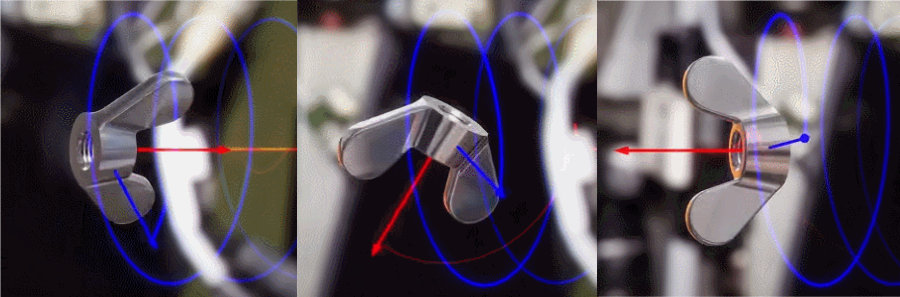
\includegraphics[width=1\textwidth]{dzhani.jpg}
\end{center}
   \caption{Dzhanibekov प्रभावको एक चित्रण \cite{28}।}
\label{fig:10}
\end{figure*}

\begin{figure*}[b]
\begin{center}
% \fbox{\rule{0pt}{2in} \rule{.9\linewidth}{0pt}}
\includegraphics[width=1\textwidth]{layers.jpg}
\end{center}
   \caption{ECDO पलटको कारण बन्ने भित्री पृथ्वीका प्रक्रियाहरूको चित्रण \cite{129}.}
\label{fig:11}
\end{figure*}

पृथ्वीको घुम्ने अक्षमा तीव्र परिवर्तन हुनुको सिद्धान्त घूर्णनशील वस्तुहरूको भौतिकशास्त्रमा आधारित छ। यसको सामान्य उदाहरण रूसी अन्तरिक्ष यात्री भ्लादिमिर जानिबेकोवद्वारा पत्ता लगाइएको जानिबेकोव प्रभाव हो \cite{37}, जुन चित्र \ref{fig:10} मा देखाइएको छ। कुनै वस्तु आफ्ना तीन प्रधान जडत्व अक्षमध्ये कुनै एकमा पूर्ण रूपमा नघुमिरहेको खण्डमा, त्यसले स्थिर घुम्ने अक्ष राख्दैन। यदि त्यो दोस्रो प्रधान अक्षको नजिकै घुमिरहेको छ भने, त्यसले अचानक घुम्ने दिशामा परिवर्तनहरू देखाउँछ। यद्यपि यो ठ्याक्कै पृथ्वीका तीव्र अक्ष पलटको समयमा हुने भन्ने हाम्रो विश्वास होइन, तर मुख्य कुरा यो हो कि बाह्य शक्तिको अभावमा, पृथ्वीको घुम्ने अक्षको तीव्र परिवर्तनलाई केवल घूर्णन भौतिकशास्त्रले मात्र व्याख्या गर्न सक्छ।

स्पष्ट रुपमा भन्ने हो भने, पृथ्वीले सायद साधारण र समान जानिबेकोव प्रभाव अनुभव गर्दैन। यदि यसो भएको भए, हामीले समयसँगै पृथ्वीको अक्षमा बिस्तारै सर्ने संकेत देख्न सक्थ्यौं। बरु, हामी विश्वास गर्छौं कि पृथ्वीले समय समयमा आफ्नो भौतिक संरचनामा अचानक अवरोधहरू अनुभव गर्छ, जसले गर्दा यसको "बाहिरी घुम्ने" (क्रस्ट/म्यान्टल) र "भित्री घुम्ने भागहरू" (कोर) अलग हुन्छन्। कुनै बाह्य प्रभाव नहुँदा, कोणीय संवेगको संरक्षणको नियमले भन्छ कि पृथ्वीले अचानक आफ्नो घुम्ने अक्ष परिवर्तन गर्न सक्दैन, त्यसैले बाहिरी र भित्री घुम्ने भागहरूको अलगाव नै, पृथ्वीमा बाह्य प्रभाव नभएमा, अचानक र तुरुन्त पलट ल्याउने थोरै चीजहरूमध्ये एक हो।
The specific process which drives the internal disruption in the Earth is believed to be a state change in the structure of iron that makes up the core of the Earth (Figure \ref{fig:11}). पृथ्वीको आन्तरिक विघटनलाई उत्प्रेरित गर्ने विशेष प्रक्रिया पृथ्वीको केन्द्र बनाउने फलामको संरचनामा हुने अवस्थात्मक परिवर्तन भएको विश्वास गरिन्छ (आकृति \ref{fig:11})। The inner core is made up of hexagonal close-packed Iron (Fe) \cite{141}. भित्री केन्द्र षट्भुज आकारका बाक्लो फलाम (Fe) ले बनेको हुन्छ \cite{141}। As this hcp-Fe is converted into a liquid metallic state, it releases kinetic energy, and is sloughed into the outer core. जब यो hcp-Fe लाई तरल धात्विक अवस्थामा रूपान्तरण गरिन्छ, यसले गतिज ऊर्जा उत्सर्जन गर्छ, र बाह्य केन्द्रमा परिणत हुन्छ। This phase change reduces the core's magnetic permeability, weakening the geomagnetic field, and releases heat, creating LLVP (large low-velocity shear province) structures (Figure \ref{fig:12}) \cite{38} in the mantle, and heating up the Earth's surface via the abyssal oceans. यो अवस्थागत परिवर्तनले केन्द्रको चुम्बकीय पारगम्यता घटाउँछ, जसले भू-चुम्बकीय क्षेत्रमा कमजोरी ल्याउँछ, र ऊष्मा उत्सर्जन गर्छ, जसले म्यान्टलमा LLVP (ठूलो न्यून-वेग कर्तन प्रदेश) संरचनाहरू (आकृति \ref{fig:12}) \cite{38} बनाउँछ, र गहिरा समुद्रहरू मार्फत पृथ्वीको सतह तताउने गर्छ। Both trends have been well documented in recent centuries and are discussed later in this paper. यी दुवै प्रवृत्तिहरू विगत शताब्दिहरूमा राम्रोसँग अभिलेख गरिएको छ र यो शोधपत्रको पछि भागमा छलफल गरिएको छ।


\begin{figure}[t]
\begin{center}
% \fbox{\rule{0pt}{2in} \rule{0.9\linewidth}{0pt}}
   \includegraphics[width=1\linewidth]{llvp.jpg}
\end{center}
   \caption{दक्षिण अफ्रिकाको मुनि रहेको LLVP को विस्तृत दृश्य \cite{28}।}

\label{fig:12}
\label{fig:onecol}
\end{figure}


यसै प्रक्रिया पृथ्वीको भित्र, उल्टो तरिकामा हुने, फ्लिप भएपछि चाँडै नै पृथ्वीको हालको घुम्ने अवस्थामा फर्कने प्रक्रियालाई पनि चलाउने विश्वास गरिन्छ।

\section{पृथ्वीको उल्टिने आसन्न प्रमाण}

\begin{figure}[t]
\begin{center}
% \fbox{\rule{0pt}{2in} \rule{1\linewidth}{0pt}}
   \includegraphics[width=1\linewidth]{npw.jpg}
\end{center}
   \caption{१५९० देखि २०२५ सम्मको भूचुम्बकीय उत्तर ध्रुवको स्थिति, ५ वर्षको अन्तरालमा देखाइएको छ \cite{142}.}
\label{fig:13}
\label{fig:onecol}
\end{figure}

हामी अर्को पृथ्वी उल्टिने घटनाको संघारमा छौँ भन्ने विश्वास गर्नको लागि बलियो कारण छ। केही सहस्राब्दीयता यता कुनै प्रलय भएको छैन, जुन ऐतिहासिक विवरण र तथ्यांकमा आधारित घटनाको आवृत्तिसँग लगभग मेल खान्छ। आसन्न उल्टिने घटनालाई समर्थन गर्ने सबैभन्दा बलियो तथ्य हालको भूचुम्बकीय विवरणबाट आएको छ, जसले देखाउँछ कि पृथ्वीको भूचुम्बकीय क्षेत्र करिब दुई हजार वर्षदेखि कमजोर हुँदै आएको छ। यो कमजोर हुने प्रक्रिया तीव्र गतिमा बढ्दो छ र केही दशकयता निकै चिन्ताजनक स्तरमा पुगेको छ।
चित्र \ref{fig:14} मा पृथ्वीको भू-चुम्बकीय क्षेत्र १५९० र २०२५ को लागि देखाइएको छ \cite{125,126}। चित्रमा देखिए अनुसार, क्षेत्र उल्लेखनीय रूपमा कमजोर भएको छ।

भू-चुम्बकीय क्षेत्र कमजोर भएको अर्को मापन सूचक भू-चुम्बकीय उत्तर ध्रुवको स्थिति हो (चित्र \ref{fig:13})। भू-चुम्बकीय उत्तर ऐतिहासिक रूपमा क्यानाडाको आर्कटिकमा अबस्थित रहेको छ। तर, यो पछिल्ला केही शताब्दीहरूदेखि बिस्तारै सर्दै आएको छ, र केही दशकअघि उल्लेखनीय रूपमा छिटो सर्दाे भएको छ। अहिले यो प्रति वर्ष ५५ किलोमिटरको दरमा छिटो रुसतर्फ गइरहेको छ \cite{124}।

\begin{figure*}[t]
\begin{center}
% \fbox{\rule{0pt}{2in} \rule{.9\linewidth}{0pt}}
\includegraphics[width=0.9\textwidth]{saa.jpg}
\end{center}
   \caption{१५९० देखि २०२५ सम्म कमजोर हुँदै गएको भूचुम्बकीय क्षेत्रको चित्रण। gufm1 र IGRF-14 मोडेलहरू प्रयोग गरी गणना गरिएको \cite{125,126}।}
\label{fig:14}
\end{figure*}

\begin{figure}[t]
\begin{center}
% \fbox{\rule{0pt}{2in} \rule{1\linewidth}{0pt}}
   \includegraphics[width=1\linewidth]{ocean-highlight.jpg}
\end{center}
   \caption{१९९१ देखि २०१० सम्म गहिरो (२००० मिटरभन्दा बढी गहिराइ) समुद्र तताउने दरहरू, रातो घेरामा देखाइएको \cite{132}।}
\label{fig:15}
\label{fig:onecol}
\end{figure}

पृथ्वीको चुम्बकीय क्षेत्र आन्तरिक डायनामोद्वारा उत्पन्न भएको विश्वास गर्न सकिन्छ - पृथ्वीको घुमाइका कारण बाहिरी कोरमा बग्ने म्याग्मा धाराका गोलाकार स्तम्भहरू \cite{123}। कमजोर हुँदै गएको भूचुम्बकीय क्षेत्र पृथ्वीको भित्री भागमा गहिरो समस्याहरूको लक्षण हो। ECDO सिद्धान्त अनुसार, यी समस्याहरूले ताप निकाल्छन् र अन्ततः म्यान्टल र कोरको छुट्टावको कारण बन्छन्, जसले पृथ्वी पल्टिन्छ \cite{1}।

पृथ्वीको भित्री भागमा भइरहेको उष्माक्षेपी प्रक्रियाहरूको उपस्थिति पुष्टि गर्ने प्रशस्त तथ्यांक उपलब्ध छन्। पृथ्वी तातो हुँदै गएको छ भन्ने कुरा महादेशीय र महासागरीय सतह तापक्रम बढ्दै गएको \cite{127,128}, पृथ्वीका तापीय ज्वालाहरूसँग तालमेल मिलाउँदै गएको वायुमण्डलीय $CO_2$ स्तर बढ्दै गएको \cite{129,130}, र विश्वव्यापी समुद्री बरफको क्षेत्रफल घट्दै गएको \cite{131} बाट देखिन्छ। तथ्यांकले देखाउँछ कि बढ्दो $CO_2$ स्तर र तापक्रमहरू "मानव-निर्मित" जलवायु परिवर्तनको कारण होइनन्, बरु एक उष्माक्षेपी कोरको परिणामस्वरूप भएका प्रभावहरू हुन् \cite{129}।

झनै महत्वपूर्ण कुरा, गहिरो महासागर (गहिराइ $>$2000 मिटर) मा तातो हुने दरहरूको अध्ययनले देखाउँछ कि न केवल गहिरा समुद्र तातो हुँदैछन्, सबैभन्दा तिव्र तातो दरहरू एबिसल तह (4000-6000 मिटर) मा पाइन्छन्। यो गहिरो सागरको तातो केन्द्र 4000 मिटरभन्दा तल छ \cite{132,129}, जुन यदि महासागरहरू माथिबाट वायुमण्डलद्वारा तातो पारिन्थ्यो भने सम्भव हुने थिएन। यस्तो तथ्यांकले पृथ्वीको भित्री प्रक्रियाहरूले हालको जलवायु र भूचुम्बकीय परिवर्तनहरू चलाएका छन् भन्ने कुरामा बलियो आधार प्रदान गर्छ। चित्र \ref{fig:15} मा १९९१ देखि २०१० सम्मको विश्वव्यापी गहिरो-सागर तातो दरहरू देखाइएको छ \cite{132}।
\section{आगामी पृथ्वीको उल्ट्याउने मोडलिङ}

\begin{figure}[t]
\begin{center}
% \fbox{\rule{0pt}{2in} \rule{1\linewidth}{0pt}}
   \includegraphics[width=1\linewidth]{saa-crop.jpeg}
\end{center}
   \caption{दक्षिण एट्लान्टिक असामान्यता मा आधारित एक टिपिङ पोइन्ट गणना अनुसार मिति मार्च १३, २०५९ आउँछ \cite{125,126}।}
\label{fig:16}
\label{fig:onecol}
\end{figure}

पृथ्वीको अर्को पल्टिने समयको पूर्वानुमान गर्नु जटिल कार्य हो। हाल, हामीसँग यसको लागि सबैभन्दा राम्रो मोडेल पृथ्वीको भू-चुम्बकीय क्षेत्र - दक्षिण एटलान्टिक असामान्यता (SAA) मा छ। दक्षिण एटलान्टिक माथिको यो क्षेत्रमा सबैभन्दा कमजोर भू-चुम्बकीय क्षेत्र बल छ र यसलाई ३२,००० न्यानोटेस्ला भन्दा कम क्षेत्र बल भएका क्षेत्रको रूपमा परिभाषित गरिएको छ \cite{135}, जुन सन् १५९० मा सबैभन्दा कमजोर क्षेत्र मान थियो। दक्षिण एटलान्टिक असामान्यता क्षेत्रको सतह क्षेत्रफल सन् १५९० मा पृथ्वीको १\% बाट २०२५ मा २१\% सम्म बढेको छ \cite{136}।

पृथ्वी कहिले पल्टिन सक्छ भन्ने अनुमान गर्नका लागि, मैले SAA सतह फैलावट डेटा पावर-ल नियम टिपिङ पोइन्ट समीकरणमा फिट गरेँ, जसले एक जटिल प्रणालीलाई एक निर्णायक संक्रमणको नजिक पुग्दै गर्दा मोडेल गर्छ, जहाँ प्रणाली अचानक र नाटकीय रूपले परिवर्तन हुन्छ। मेरो गणनामा, भविष्यवाणी गरिएको टिपिङ पोइन्ट मिति मार्च १३, २०५९ (चित्र \ref{fig:16}) आएको छ। हामी संक्रमणको झन् नजिकिन जाँदा यो भविष्यवाणी झन् झन् सटीक बन्दै जान्छ \cite{136}।

अन्य मापदण्डहरूसम्मेत जस्तै घूर्णन अक्ष विचलन, मौसम असामान्यता, र भूकम्प तथा ज्वालामुखी डेटा समेतले हामीलाई पृथ्वीको अर्को पल्टिने समयको अझ राम्रो पूर्वानुमान गर्न मद्दत गर्न सक्छ।

\section{ECDO ऐतिहासिक समयरेखा}
While establishing an exact timeline for past ECDO events is difficult, it seems that there were at least 2 ECDO events during the Holocene. Note the account told by Herodotus from Egyptian priests that, \textit{"पहिलो राजाबाट लिएर अन्तिमपटक शासन गरेको हेफाइसटोसका याजकसम्म तीन सय बयालीस पुस्ता मानवहरुको भएको... यस समयमा उनीहरूले भने कि सूर्यले चार पटक आफ्नो नियमित उदाउँने स्थान सरेको थियो, र जहाँ अहिले अस्ताउँछ, त्यहाँबाट दुई पटक उदाएको थियो, र जहाँ अहिले उदाउँछ, त्यहाँ दुई पटक अस्ताएको थियो"} \cite{32}। प्लेटो, जो पाँचौं शताब्दी ईसा पूर्वमा बस्थे \cite{111}, ले भनेका थिए कि अटलांटिस एकै दिन र रातमा डुवाएको बाढीपछि ९,००० वर्ष अघिदेखि \textit{"त्यसपछि धेरै बाढीहरु आएको छ, र पहाडमा बाँचेकाहरू लेखन कलाबाट अनविज्ञ थिए, र धेरै पुस्ताहरू बाँच्नका लागि आवश्यक सीपहरू सिक्नमै लागेका थिए"} \cite{112}, जसले देखाउँछ कि यंगर ड्रायासको अन्त्य (करिब ९७०० ईसापूर्व) पछि दुईभन्दा बढी पलट भएका थिए। यस लेख र मेरो अनुसन्धानमा समावेश भौतिक प्रमाणहरूले प्लेटोको कथनलाई पर्याप्त समर्थन दिन्छ \cite{2}।

हालसम्मको सबैभन्दा नजिकको सम्भाव्य ईसीडीओ पलटको मिति २३०० देखि १६०० ईसापूर्वको कालखण्डमा पर्छ, जसमा धेरै विपद्कर बाढी कथाहरू (गुन-यू \cite{113,114,115}, ओग्यजेस \cite{116,117}, पेरु \cite{118,119}, प्रस्थान \cite{120}), सभ्यताको विनाश तथा परित्याग (मोहेन्जोदरो \cite{121}, मिनोअन क्रिट \cite{100,101}) र भौतिक असमानताहरु (बन्ड इभेन्ट्स \cite{122}, ४.२ किलोवर्ष घटना \cite{90}) मिति नियन्त्रण गरिएको छ। यसपछिको कालदेखि नयाँ कुनै ठूला विनाशकारी घटनाको पर्याप्त प्रमाणको जम्काभेट छैन।

\section{निष्कर्ष}

अप्रेशन NANOOK दोस्रो विश्वयुद्धपछि संयुक्त राज्य अमेरिकाद्वारा आर्कटिक र सोभियत उत्तरतटको नक्साङ्कनका लागि गरिएको चिसोयुद्धकालीन अन्वेषण अभियान थियो \cite{137}। उनीहरूको अनुसन्धानको क्रममा, पहिलेका अन्वेषणहरूमा आधारित अनुमानको तुलनामा चुम्बकीय ध्रुव १२५ देखि २०० माइल उत्तर तिर भेटिएको थियो। त्यसैले, \textit{"सरकारी वैज्ञानिकहरू बीच प्रश्न उठ्यो कि जब चुम्बकीय र भौगोलिक ध्रुवहरू एउटै स्थानमा आइपुग्छन् भने के हुन्छ। यसको उत्तरका लागि, डा. पाउल ए. सिपलको प्रोजेक्ट नियन्त्रणमा, र्यान्ड कर्पोरेशनलाई पृथ्वीको केन्द्र-केंद्रित गोला मोडेलहरू प्रयोग गरी प्रयोगशाला अध्ययन गर्न ठेक्का दिइयो—भित्रको गोला विद्युत् चुम्बकीय लोहा कोरलाई जनाउने, जसको अक्षले 'चुम्बकीय' ध्रुव परिभाषित गर्थ्यो; र बाहिरी गोला पृथ्वीको क्रस्टलाई जनाउने, जुन 'भौगोलिक' ध्रुवीय अक्ष वरिपरि घुम्थ्यो। पटक–पटकको प्रयोगबाट पत्ता लाग्यो कि 'चुम्बकीय' ध्रुव 'भौगोलिक' ध्रुव नजिकिंदै जाँदा, एउटा बिन्दुमा पुगेर चुम्बकीय ध्रुवले भौगोलिक ध्रुवतिर आकर्षित भएर उसको गति अचानक बढाउँछ र एकैचोटी भिड्न पुग्छ; तर ध्रुवहरू मिल्ने सट्टा, 'चुम्बकीय' ध्रुव छिट्टै 'भौगोलिक' ध्रुव वरिपरि घुम्छ र केन्द्रीय बलले फ्याकिएजस्तै भूमध्यरेखा तिर जान्छ, जसको अन्त्यमा यी दुई अक्षहरू लगभग ८९ डिग्रीले छुट्टिएको अवस्थामा रहन्छन्। यो ध्रुवीय 'पलट' भएको पछि, समयक्रमसँगै यी अक्षहरू फेरि बिस्तारै एकअर्कातिर फर्कन थाल्छन्"} \cite{138,139}।

त्यसपछि, \textit{"१९४८ को प्रारम्भतिर पेन्टागनमा मेजर ह्वाइटले सहभागी भएको वैज्ञानिक बैठकमध्ये एउटामा, वैज्ञानिकहरूले चाँडै आउने ध्रुवीय-पलट घटनाको सन्दर्भमा जनतालाई सतर्क गराउने सल्लाह–विवेकबारे छलफल गरे। कुनै पनि वैज्ञानिकले जनतालाई जानकारी नदिने प्रस्तावमा सहमति जनाएनन्; तर, अर्कोतर्फ, कुनैले कसरी जानकारी दिने भन्नेमा पनि सहमति जताएनन्। केहि वैज्ञानिकलाई लाग्यो, यस घटनाको ज्ञानले नै समाजको नैतिक धारणा नष्ट गर्न सक्छ। तर, उनीहरूको डर निराधार प्रमाणित भयो, जब १९५० को दशकको सुरुतिर, पलट घटनाको जानकारी पत्रिका र पत्रिका दुवैमा प्रकाशित भयो, तर आश्चर्यजनकरूपमा स्तब्ध, स्थानीय वा अविश्वासी जनताबाट कुनै प्रतिक्रिया आएन"} \cite{138,139}।
Why are we not paying attention to this? There is ample reason to believe that the Earth has flipped before. This paper, along with part two of the paper, provide a dense summary of a great convergence of evidence from many areas suggesting that this is the case, such as flood stories all over the world, salt and marine fossils covering the continents, ancient underground shelters, animal remains, and cataclysmic geological landscapes. Humans are supposedly hundreds of thousands of years old, yet modern history only goes back several thousand years. Might it not be the case that every so often, the Earth flips, the continents are wiped clean, and we are forced to return to square one - the Stone Age - reducing our records of ancient history to a handful of cataclysmic stories? If so, then preventing this from happening again may be one of humanity's most important tasks.

In closing, I shall leave you with this account recounted in Timaeus, written by Plato, of a conversation between Solon, an Athenian statesman, and Egyptian priests \cite{140}: \textit{"And on one occasion, when [Solon] wished to draw them on to discourse on ancient history, he attempted to tell them the most ancient of our traditions, concerning Phoroneus, who was said to be the first man, and Niobe; and he went on to tell the legend about Deucalion and Pyrrha after the Flood, and how they survived it, and to give the geneology of their descendants; and by recounting the number of years occupied by the events mentioned he tried to calculate the periods of time. Whereupon one of the priests, a prodigiously old man, said, “O Solon, Solon, you Greeks are always children: there is not such a thing as an old Greek.” And on hearing this he asked, “What mean you by this saying?” And the priest replied, “You are young in soul, every one of you. For therein you possess not a single belief that is ancient and derived from old tradition, nor yet one science that is hoary with age. And this is the cause thereof: There have been and there will be many and divers destructions of mankind, of which the greatest are by fire and water, and lesser ones by countless other means. For in truth the story that is told in your country as well as ours, how once upon a time Phaethon, son of Helios, yoked his father's chariot, and, because he was unable to drive it along the course taken by his father, burnt up all that was upon the earth and himself perished by a thunderbolt — that story, as it is told, has the fashion of a legend, but the truth of it lies in the occurrence of a shifting of the bodies in the heavens which move round the earth, and a destruction of the things on the earth by fierce fire, which recurs at long intervals. At such times all they that dwell on the mountains and in high and dry places suffer destruction more than those who dwell near to rivers or the sea; and in our case the Nile, our Saviour in other ways, saves us also at such times from this calamity by rising high. And when, on the other hand, the Gods purge the earth with a flood of waters, all the herdsmen and shepherds that are in the mountains are saved, but those in the cities of your land are swept into the sea by the streams; whereas In our country neither then nor at any other time does the water pour down over our fields from above, on the contrary it all tends naturally to well up from below. Hence it is, for these reasons, that what is here preserved is reckoned to be most ancient; the truth being that in every place where there is no excessive heat or cold to prevent it there always exists some human stock, now more, now less in number. And if any event has occurred that is noble or great or in any way conspicuous, whether it be in your country or in ours or in some other place of which we know by report, all such events are recorded from of old and preserved here in our temples; whereas your people and the others are but newly equipped, every time, with letters and all such arts as civilized States require and when, after the usual interval of years, like a plague, the flood from heaven comes sweeping down afresh upon your people, it leaves none of you but the unlettered and uncultured, so that you become young as ever, with no knowledge of all that happened in old times in this land or in your own. Certainly the genealogies which you related just now, Solon, concerning the people of your country, are little better than children's tales; for, in the first place, you remember but one deluge, though many had occurred previously; and next, you are ignorant of the fact that the noblest and most perfect race amongst men were born in the land where you now dwell, and from them both you yourself are sprung and the whole of your existing city, out of some little seed that chanced to be left over; but this has escaped your notice because for many generations the survivors died with no power to express themselves in writing. For verily at one time, Solon, before the greatest destruction by water, what is now the Athenian State was the bravest in war and supremely well organized also in all other respects. It is said that it possessed the most splendid works of art and the noblest polity of any nation under heaven of which we have heard tell”}.

These same priests, of course, also told Solon about the ancient civilization of Atlantis: \textit{"For all that we have here, lying within the mouth of which we speak, is evidently a haven having a narrow entrance; but that yonder is a real ocean, and the land surrounding it may most rightly be called, in the fullest and truest sense, a continent. Now in this island of Atlantis there existed a confederation of kings, of great and marvellous power, which held sway over all the island, and over many other islands also and parts of the continent; and, moreover, of the lands here within the Straits they ruled over Libya as far as Egypt, and over Europe as far as Tyrrhenia. So this host, being all gathered together, made an attempt one time to enslave by one single onslaught both your country and ours and the whole of the territory within the Straits. And then it was, Solon, that the manhood of your State showed itself conspicuous for valor and might in the sight of all the world. For it stood pre-eminent above all in gallantry and all warlike arts, and acting partly as leader of the Greeks, and partly standing alone by itself when deserted by all others, after encountering the deadliest perils, it defeated the invaders and reared a trophy; whereby it saved from slavery such as were not as yet enslaved, and all the rest of us who dwell within the bounds of Heracles it ungrudgingly set free. But at a later time there occurred portentous earthquakes and floods, and one grievous day and night befell them, when the whole body of your warriors was swallowed up by the earth, and the island of Atlantis in like manner was swallowed up by the sea and vanished"}.

\section{Acknowledgments}

Thanks to Ethical Skeptic, the original author of the ECDO thesis, for completing his insightful, groundbreaking thesis and sharing it with the world. His tri-part thesis \cite{1} remains the seminal work for Exothermic Core-Mantle Decoupling Dzhanibekov Oscillation (ECDO) theory, and contains much more information on the topic than I have covered briefly here.

---

किन हामीले यसतर्फ ध्यान दिइरहेका छैनौं? पृथ्वी पहिले पनि पल्टिएकोमा विश्वास गर्न पर्याप्त कारण छ। यस पत्रिकाले, साथै पत्रिकाको दोस्रो भागले, यो कुरा संकेत गर्ने धेरै क्षेत्रहरुबाट आएको प्रमाणहरुको ठूलो संगमको घना सारांश दिन्छ, जस्तै संसारभरको बाढीका कथाहरू, महाद्वीपहरू ढाक्ने नून र समुद्री जीवाश्महरू, प्राचीन भूमिगत आश्रयहरू, जनावरका अवशेषहरू, र विनाशकारी भू-परिदृश्यहरू। भनिन्छ, मानिसहरु सयौं हजारौं वर्ष पुराना हुन्, तर आधुनिक इतिहास केही हजार वर्ष मात्र पछाडि जान्छ। के हरेक केहि समयपछि पृथ्वी पल्टने, महाद्वीपहरू सफा गरिने, र हामी फेरि शून्य, अर्थात् पत्थर युगमा फर्किन बाध्य हुने, जसले गर्दा प्राचीन इतिहासका अभिलेखहरू केही थोरै विनाशकारी कथामा सीमित हुने त होइन? यदि हो भने, यो पुनः हुन नदिने काम मानवताको सबैभन्दा महत्वपूर्ण जिम्मेवारीमध्ये एक हुनसक्छ।

अन्त्यमा, तपाईँलाई प्लेटोले लेखेको टिमायसमा प्रस्तुत गरिएको, एथेन्सका राजनेता सोलन र इजिप्टका पुजारिहरूबीचको संवाद यहाँ प्रस्तुत गर्न चाहन्छु \cite{140}: \textit{"र एकपटक, जब [सोलन] तिनीहरूलाई प्राचीन इतिहासको चर्चा गर्न इच्छुक थिए, उनले हाम्रा सबैभन्दा प्राचीन परम्पराहरू सुनाउने प्रयास गरे, जहाँ फरोनियसलाई पहिलो मानिस भनिन्थ्यो, अनि नायोब; अनि उनले ड्यूकेलियन र पिर्राको बाढीपछिको किंवदन्ती सुनाए, र कसरी उनीहरूले त्यसबाट जोगिए, अनि तिनका सन्तानहरूको वंशावली दिएका; अनि उल्लेख गरिएका घटनाहरूका वर्षहरू गन्ने प्रयास गरे। त्यतिबेला पूराना पुजारीमध्ये एकजनाले भने, “ओ सोलन, सोलन, तिमीहरु ग्रीकहरू सधैं बच्चा हौ: त्यहाँ कुनै पुरानो ग्रीक हुँदैन।” उनले यो सुनी सोधे, “यस भनाइको के अर्थ हो?” अनि त्यस पुजारीले भने, “तिमीहरु सबै आत्मामा जवान हौ। यहाँ कुनै प्राचीन विश्वास छैन, परम्पराबाट आएको; न त कुनै विज्ञान नै, जुन परम्परागत होस्। यसको कारण हो: मानव सभ्यताको धेरै विनाश भएका छन्, र हुन्दै जानेछन्, जसमा सबैभन्दा ठूलो आगो र पानीबाट हुने हो, अनि कम ती अन्य अनगिन्ती तरिकामा हुने छन्। तिमीहरुका देश र हाम्रामा सुनिने कथा, पायथन, हेलिओसका छोरा, जसले बुबाको रथ चलाउन सकेन र सब जलेर मरे — त्यो कथा किंवदन्तीजत्रो लाग्छ, तर यसको सत्यता भने स्वर्गका शरीरहरूको स्थानान्तरणमा छ, अनि पृथ्वीका वस्तुको ध्वंसमा, जुन लामो अन्तरालमा पुनः हुन्छ। यस्ता समयमा पहाड र उचाइका सूखा ठाउँका बासिन्दा नदी वा समुद्र नजिकका भन्दा बढी विनाशमा पर्छन्; हाम्रामा नाइल नदी, अरू तरीकाले जस्तो, त्यस्ता समयमा यस प्रकोपबाट उचालिएर बचाउँछ। अनि जब जलप्रलय हुन्छ, पर्वतका गोठाला र बाख्रापालक बच्छन्, तर तिम्रो देशका सहरहरूका मानिसहरू नदीको बहावले समुद्रमा बगाउँछन्; हाम्रामा चाहे तत् बखत होस् वा अन्य समय, माथिबाट पानी खस्दैन, बरु तलबाट उक्लिन्छ। त्यसैले यहाँ जे बाकि छ, सबैभन्दा प्राचीन मानिन्छ; साँचो कुरा जहाँ अनावश्यक गर्मी वा चिसो छैन, त्यहाँ सधैँ केही मानव जाति रहन्छ, कहिले धेरै, कहिले थोरै। कुनै कुरा जति राम्रो वा ठूलो भए पनि, तिम्रो देशमा होस् वा हाम्रामा वा अन्य सुनेका ठाउँमा, त्यसलाई यहाँका मन्दिरहरूमा राखिन्छ; जबकि तिमीहरुको पुस्ता र अरू हरेक पटक नयाँ अक्षर र कला मात्र देखाउँछ, अनि जब हरेक वर्षको अन्तरालमा, जस्तो महामारीजस्तो, आकाशको बाढी आउँछ, तिमीहरुमा शिक्षित र सुसंस्कृत कोही बाँकी रहँदैन, अनि तिमीहरु फेरि पुरानै जस्तै जवान हुन्छौ, न त यहाँको न त आफ्नै देशको प्राचीन इतिहासको कुनै ज्ञान रहन्छ। तिमीले अहिले भनेजस्तो वंशावली, सोलन, तिम्रो देशका मानिसको, बालकहरूको कथा भन्दा खास राम्रो छैन; किनभने तिमीले एक मात्रै प्रलय सम्झन्छौ, जबकि धेरै पहिल्यै भइसकेका थिए; अनि तिमीलाई थाहा छैन, सबैभन्दा राम्रो र पूर्ण जाति तिम्रो देशमै जन्मिएका थिए, र तिनबाट तिमी र तिम्रो सहर बाँकी छ; तर धेरै पुस्तासम्म लेखनको शक्ति नहुँदा बाँकीहरूले केही अभिव्यक्त गर्न सकेनन्। कुनै समयमा, सोलन, सबैभन्दा ठूलो जलप्रलयभन्दा अघि, अहिलेको एथेन्सी राज्य युद्धमा सबैभन्दा बहादुर थिए र अरू कुरामा पनि सर्वोच्च रुपमा संगठित थिए। भनिन्छ, यसले सबैभन्दा मनमोहक कला र सबभन्दा उत्कृष्ट शासन व्यस्था राख्थ्यो, जुन हामीले सुनेका छौं।”}

त्यसै पुजारीहरूले, सोलनलाई प्राचीन एटलान्टिस सभ्यताको बारेमा पनि भनेका थिए: \textit{"हामीले यहाँ जे देखेका छौं, यो सबै, खोलको भित्रको बन्दरगाह हो; तर त्यो टाढा साँचो महासागर हो, त्यसलाई पूरै महाद्वीप भन्न सकिन्छ। एटलान्टिस टापुमा प्रशंसा योग्य राजा र अद्भुत शक्तिको महासंघ थियो, जसले टापु मात्र हैन, धेरै टापुहरू, महाद्वीपका भाग नियन्त्रणमा राखेका थिए; अनि यहाँको तटकै कुरा गर्दा, तिनीहरूले लिविया, इजिप्ट र युरोपका भागसमेत शासित गरेका थिए। तिनीहरू सबै मिलेर, एकपटक, तिम्रो र हाम्रो देशलाई साथै हरक्युलिसको सिमानामा रहेको क्षेत्रलाई दास बनाउने प्रयास गरे। अनि सोलन, तिम्रो राज्यको वीरता र शक्ति सबभन्दा उजागर देखियो। सबैमा महान र युद्धकला सीपमा अग्रणी भएर, ग्रीकहरूको नेतालाई समर्थन गरेर वा अन्य सबैले छाडेपछि आफैंमा मात्र खडा भएर, खतरासँग जुधेर तिनीहरूले आक्रमणकारीहरूलाई परास्त गरे र विजय चिन्ह बनाए; जसले बाँकी नदास भएभन्दा पनि जनतालाई मुक्त गर्यो, बाँकी हामीलाई पनि हरक्युलिसको सीमाभित्र मुक्त गर्यो। तर केही समयपछि, भयंकर भूकम्प र बाढी आए र एक भयावह दिन र रात, तिम्रो सबै सैनिकहरू पृथ्वीमा बिलाए, एटलान्टिस टापु पनि समुद्रमा विलीन भई गुप्त भयो"}।

\section{Acknowledgments}

थैंक्स टू एथिकल स्केप्टिक, ईसीडीओ थेसिसका मौलिक लेखक, जसले आफ्नो अन्तर्दृष्टियुक्त, क्रान्तिकारी थेसिस पूरा गरेर संसारसित बाँडे। उनको त्रैतीय थेसिस \cite{1} अझै पनि Exothermic Core-Mantle Decoupling Dzhanibekov Oscillation (ECDO) सिद्धान्तको प्रमुख काम हो, र यस विषयमा यहाँ संक्षिप्त रूपमा उल्लेखभन्दा धेरै जानकारी समेटिएको छ।
Thanks to Ankit, who processed the cataclysm compilation data in Table 1.

र अवश्य, धन्यवाद ती दिग्गजहरूलाई जसको काँधमा हामी उभिएका छौं; ती जसले सबै अनुसन्धान र अन्वेषण गरे जसले यो कार्य सम्भव बनायो र मानवजातिलाई उज्यालो ल्याउनका लागि मेहनत गरे।

\clearpage
\twocolumn

\section{थप तस्वीरहरू}
\begin{figure}[H]
\begin{center}
% \fbox{\rule{0pt}{2in} \rule{1\linewidth}{0pt}}
   \includegraphics[width=1\linewidth]{wave.jpg}
\end{center}
   \caption{खफ्रे पिरामिडमा रहेको अन्डरकट, प्याराबोलिक तरंगीय क्षयरूपमा नजिकबाट गरिएको अवलोकन \cite{27}.}
\label{fig:19}
\label{fig:onecol}
\end{figure}

\begin{figure}[H]
\begin{center}
% \fbox{\rule{0pt}{2in} \rule{1\linewidth}{0pt}}
   \includegraphics[width=1\linewidth]{star-stone.jpg}
\end{center}
   \caption{खुफु पिरामिडका शाफ्टमध्ये एउटामा पत्थरमा कुँदिएको ताराकाे नक्सा \cite{28}।}
\label{fig:20}
\label{fig:onecol}
\end{figure}
\begin{figure*}[t]
\begin{center}
% \fbox{\rule{0pt}{2in} \rule{.9\linewidth}{0pt}}
\includegraphics[width=1\textwidth]{deepsea.jpg}
\end{center}
   \caption{सामान्य वायुमण्डलीय महासागर तताउने वक्रको तुलना गर्दा गहिरो र अतिगहिरो महासागर तताउने असमानतालाई देखाउने दृश्य। समग्र तताउने असमानता NOAA बाट लिइएको हो \cite{147}, गहिरो र अतिगहिरो तताउने वितरणहरू Desbruyeres अध्ययनबाट \cite{132}, र डेटा प्रशोधन तथा दृश्यांकन Ethical Skeptic द्वारा \cite{129}।}
\label{fig:21}
\end{figure*}

\begin{figure*}[t]
\begin{center}
% \fbox{\rule{0pt}{2in} \rule{.9\linewidth}{0pt}}
\includegraphics[width=1\textwidth]{sealevel.jpeg}
\end{center}
   \caption{समुद्री सतहले ७५ वर्षमा ६३ वटा स्टेसनहरूमा २०\% भेरियन्सको वृद्धि देखाउँछ, जसले हालको गतिमा बृद्धि भएको देखाउँछ। समुद्री सतहको भेरियन्समा आएका तीव्र वृद्धिहरू महासागरको तापमान वृद्धि सँगै देखिन्छन्, जसले यी दुवै कारण पृथ्वीको गहिराइबाट उत्पन्न तापका कारण हुन सक्छन् भन्ने संकेत गर्छ \cite{2,129}।}
\label{fig:22}
\end{figure*}

\begin{figure*}[t]
\begin{center}
% \fbox{\rule{0pt}{2in} \rule{.9\linewidth}{0pt}}
\includegraphics[width=1\textwidth]{co2.jpg}
\end{center}
   \caption{गत ४५ वर्षमा वायुमण्डलीय CO2 ppm स्थायी रूपमा वृद्धि भएको छ, सम्भवतः समुद्रको तापक्रममा वृद्धिका कारण। स्रोत: NOAA \cite{148,129}.}
\label{fig:23}
\end{figure*}

\begin{figure*}[t]
\begin{center}
% \fbox{\rule{0pt}{2in} \rule{.9\linewidth}{0pt}}
\includegraphics[width=1\textwidth]{ice.jpg}
\end{center}
   \caption{पृथ्वी तात्दै गएको कारणले विश्वव्यापी समुन्द्री हिउँको क्षेत्रफल पछिल्ला ४५ वर्षमा घट्दै गएको छ। स्रोत: ADS \cite{149}.}
\label{fig:24}
\end{figure*}

\clearpage
\twocolumn

{\small
\bibliographystyle{ieee}
\bibliography{egbib}
}

\end{document}